%----------------------------------------------------------------------------
\chapter{Szerver oldal}
\label{chapt:birdmap-backend}
%----------------------------------------------------------------------------
Ebben a fejezetben bemutatom a szerveroldal architektúráját, felépítését. Ismertetem a különböző szoftver komponensek feladatát.

%----------------------------------------------------------------------------
\section{Architektúra}
%----------------------------------------------------------------------------
A szerveroldal fejlesztésénél a háromrétegú architektúrát alkalmaztam, melynek lényege, hogy az alkalmazást logikailag három elkülönülő részre bontjuk:
\begin{itemize}
    \item \textbf{Adat elérési réteg}. Ez a rész felel a tárolt entitások modell definícióiért, illetve azoknak a kiolvasásáért, tárolásáért egy adatbázisból vagy fájlrendszerből.
    \item \textbf{Megjelenítési réteg}. Ezen réteg feladata a kliensoldal közvetlek kiszolgálása. Bármilyen irányú kommunikáció a kliensek felé ezen a rétegen keresztül történik.
    \item \textbf{Üzleti logikai réteg}. Minden ami nem a közvetlen kommunikációért, megjelenítésért vagy adat elérésért, tárolásért felel, az ide kerül.
    A fenti két réteg között helyezkedik el és feladata a különböző folyamatok értékelése és futtatása, valamint az adatok feldolgozása.
\end{itemize}

Az ASP.NET Core beépítetten támogatja a dependency injection-t, mely a \verb+Startup+ osztály \verb+ConfigureServices+ metódusával konfigurálható.
Én minden rétegbe tettem egy ilyen \verb+Startup+ osztályt, hogy azok feleljenek a saját szolgáltatásaik konfigurálásáért és regisztrálásáért.

%----------------------------------------------------------------------------
\section{Adat elérési réteg}
%----------------------------------------------------------------------------
Az adatelérést az Entity Framework Core segítségével oldottam meg. Telepítettem egy MSSQL adatbázis szervert a számítógépemre, melynek csatlakozási paramétereivel
a \verb+Startup+ osztályban felkonfigurálom az EF Core által nyújtott \verb+DbContext+ saját leszármazott változatát. 
Így csak az entitások elkészítése és azok alapértelmezett értékeinek az adatbázisba való feltöltése marad hátra.

%----------------------------------------------------------------------------
\subsection{Entitások}
%----------------------------------------------------------------------------
Mivel az adatok nagy részét külső szolgáltatások fogják nyújtani, így lokálisan összesen két entitás létrehozására volt szükség. 
Az egyik a \verb+User+, mely az alkalmazás felhasználóinak adatait tárolja. 
A másik a \verb+Service+, mely a külső szolgáltatások adatainak tárolását szolgálja, amelyeket azért tárolok az adatbázisban és nem mondjuk a konfigurációs fájlban,
mert szerettem volna, hogyha a kezelőfelületen lehetne őket szerkeszteni, törölni.

\lstset{style=sharpc, morekeywords={record, get, set}}
\begin{lstlisting}[caption=A User és a Service modell]
    public record User
    {
        public int Id { get; set; }
        public string Name { get; set; }
        public byte[] PasswordHash { get; set; }
        public byte[] PasswordSalt { get; set; }

        public Roles Role { get; set; }

        public bool IsFromConfig { get; set; }
    }

    public record Service
    {
        public int Id { get; set; }
        public string Name { get; set; }
        public Uri Uri { get; set; }

        public bool IsFromConfig { get; set; }
    }
\end{lstlisting}

Az alkalmazás használata szempontjából a felhasználók két csoportba oszlanak.
Vannak adminisztrátor és sima felhasználók, utóbbi csak az adatok olvasására, míg előbb azok módosítására is jogosult.
A \verb+Role+ mező ennek a megkülönböztetsnek a jelzője.

%----------------------------------------------------------------------------
\subsection{Seedelés}
\label{subsect:seeding}
%----------------------------------------------------------------------------
Az alkalmazás konfigurációs fájljából meg lehet adni alapértelmezett felhasználókat és szolgáltatásokat.
Ezeknek megkülönböztetésére szolgál az entitások \verb+IsFromConfig+ mezője.
A szerver indítása legelején, megvizsgálja, hogy létezik-e az adatbázis és ha igen kitöröl minden olyan entitást ahol az \verb+IsFromConfig+ mező igaz.
Majd hozzáadja az újonnan beolvasott értékeket.

%----------------------------------------------------------------------------
\section{Üzleti logikai réteg}
%----------------------------------------------------------------------------
Ebben a rétegben található meg a szerver legtöbb szolgáltatása. It vannak implementálva a Birdnetes Command and Control és Input komponensekkel kommunikáló szolgáltatások is, 
melyeket azok OpenAPI leírói alapján az NSwag\cite{nswag} alkalmazással generáltam. Az OpenAPI a klienseken kívül definiálja még az azok által használt modelleket is.
A Command and Control által használt \verb+Device+ modell tartalmazza annak egyedi azonosítóját, státuszát, koordinátáit és a használt szenzorok listáját, 
melyeknek szintén van egy modellje \verb+Sensor+ néven. Ennek szintén van azonosítója és státusza. Az Input szolgáltatásnak is van saját modellje, 
amely a hangüzenetek metaadatait reprezentálja. Többek között tartalmazza a kihelyezett eszköz egyedi azonosítóját és a hangüzenet keltének dátumát. 

Ugyan itt található meg a \verb+User+ és \verb+Service+ entitások létrehozásáért, olvasásáért, szerkesztéséért és törléséért felelős szolgáltatások is.
Valamint itt található még az autentikációért felelős szolgáltatás is. A felhasználók jelszavainak tárolására a HMAC (Hash-based Message Authentication Code) algorithmust, 
pontosabban annak a \verb+HMACSHA512+\cite{hmacsha512} C\# implementációját használtam.

Minden jelszóhoz generálok egy egyedi kulcsot és azzal egy hash-t, majd ezeket tárolom a \verb+User+ modell \verb+PasswordSalt+ és \verb+PasswordHash+ mezőiben.
Amikor egy felhasználó be akar jelentkezni először megvizsgálom, hogy egyáltalán létezik-e az adatbázisban az adott nevű felhasználó, 
ha igen, akkor a megadott jelszóból az imént említett folyamattal generált kulcsot és hash-t összehasonlítom az adatbázisban tárolttal.

%----------------------------------------------------------------------------
\section{Megjelenítési réteg}
%----------------------------------------------------------------------------
A fejezet elején említett \verb+Startup+ osztály ebben a rétegben található, itt kerülnek az egyes szolgáltatások regisztrálásra.
Itt történik a \ref{subsect:seeding} fejezetben leírt adatbázis seedelése is.

Többek között a naplózás is itt kerül inicializálásra, mely az NLog saját konfigurációs fájljával történik.
Meg lehet adni különböző szűrőket és kimeneteket, amellyel szelektálni lehet, hogy az egyes naplózott események hova kerüljenek.
Például az MQTT szolgáltalás napló bejegyzéseit a \ref{lst:nlog-config} lista alapján szűrtem.
Minden \verb+Debug+ szintől nagyobb és \verb+Error+ szinttől kisebb bejegyzés, mely tartalmazza az \verb+Mqtt+ kulcsszót az \verb+mqttFile+ azonosítójú fájlba kerül.

\lstset{style=xml, morekeywords={targets, target, xsi:type, name, fileName, layout, rules, logger, name, minlevel, maxlevel, writeTo, final}}
\begin{lstlisting}[caption=Az NLog.config fájl egy részlete, label=lst:nlog-config]
<targets>
    ...
    <target xsi:type="File" name="mqttFile" fileName="${basedir}Logs/birdmap-mqtt-${shortdate}.log"
        layout="..." />
    ...
</targets>

<rules>
    ...
    <logger name="*.*Mqtt*.*" minlevel="Trace" maxlevel="Warning" writeTo="mqttFile" final="true"/>
    ...
</rules>
\end{lstlisting}

A \verb+Startup+ osztály másik metódusa a \verb+Configure+, mellyel a HTTP kérések csővezetéke konfigurálható.
Azaz, hogy egy kérés-t milyen sorrendben dolgozzák fel a regisztrált szolgáltatások.
A szerveroldali kivételkezelésre szánt szolgáltatás, az \verb+ExceptionHandlerMiddleware+ is itt van használva, 
amely elkap minden kivételt, amit a csővezeték további részei dobtak és JSON formátumban visszaadja azokat a kliensnek.

Továbbá az NSwag\cite{nswag} szoftvercsomag segítségével regisztrálok egy szolgáltatást, 
mely a szerveroldalon található kontrollereket felhasználva generál egy OpenAPI specifikációt és annak egy Swagger UI\cite{swagger-ui} felületet,
ahol a végpontok kipróbálhatóak, tesztelhetőek kliensoldal nélkül is.

\begin{figure}[!ht]
    \centering
    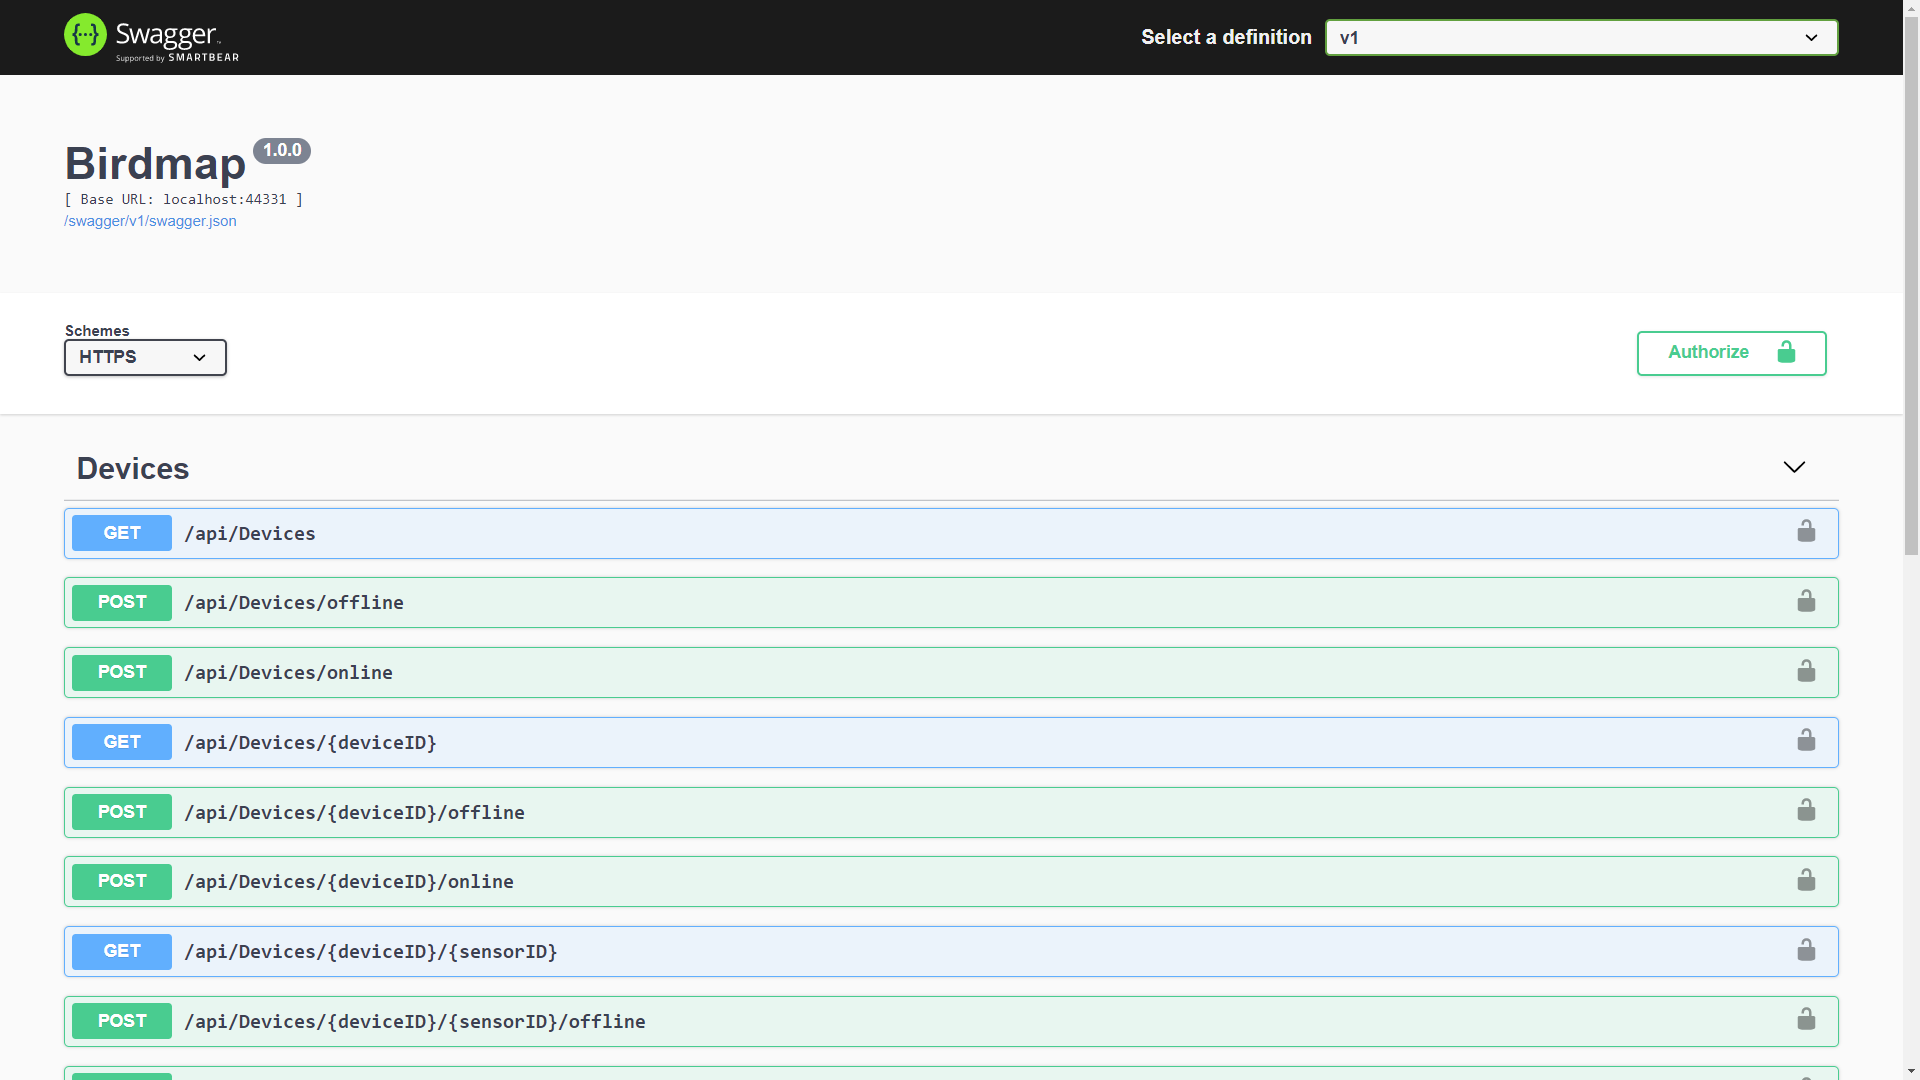
\includegraphics[width=150mm, keepaspectratio]{figures/swagger-ui.png}
    \caption{Az alkalmazásom Swagger felülete}
    \label{fig:swagger-ui}
\end{figure}

%----------------------------------------------------------------------------
\subsection{Kommunikációs Szolgáltatások}
%----------------------------------------------------------------------------
A kliensoldal frissítésére több megoldás is létezik. Például bizonyos időközönként lehetne kéréseket indítani a szerver felé a friss adatok megszerzéséért.
Egy másik megoldás a SignalR használata, amellyel a klienseket eseményvezérelten lehet értesíteni, megvalósítja a kétoldalú kommunikációt.
Így a kliensek csak akkor indítanak kéréseket amikor az adat tényleg változott. Ezzel a technológiával oldottam meg például, hogy az eszközök állapotainak változására
frissüljön a felület.

Egy másik szolgáltatás a Birdnetes MQTT kommunikációért felelős szolgáltatás, 
mely felregisztrál a \ref{subsect:birdnetes-ai-service}-as alfejezetben bemutatott AI Service által publikált üzenetekre.
Ezekben az üzenetekben található a hanganyagok egyedi azonosítója, illetve azok seregélytől való származásának valószínüsége.
Ha a szolgáltatás kap egy ilyen üzenetet akkor lekérdezi a \ref{subsect:birdnetes-input-service}-es alfejezetben bemutatott Input Service-től
a hanganyag azonosítójához tartozó metaadatokat. 
Ezekből felhasználva a kihelyezett eszköz azonosítóját, a hanganyag beérkezésének dátumát és az említett valószínüséget új üzeneteket készítek, melyeket egy pufferben tárolok.
Ezt a folyamatot a \ref{fig:birdmap-mqtt-service}-es ábra szemlélteti.

\begin{figure}[!ht]
    \centering
    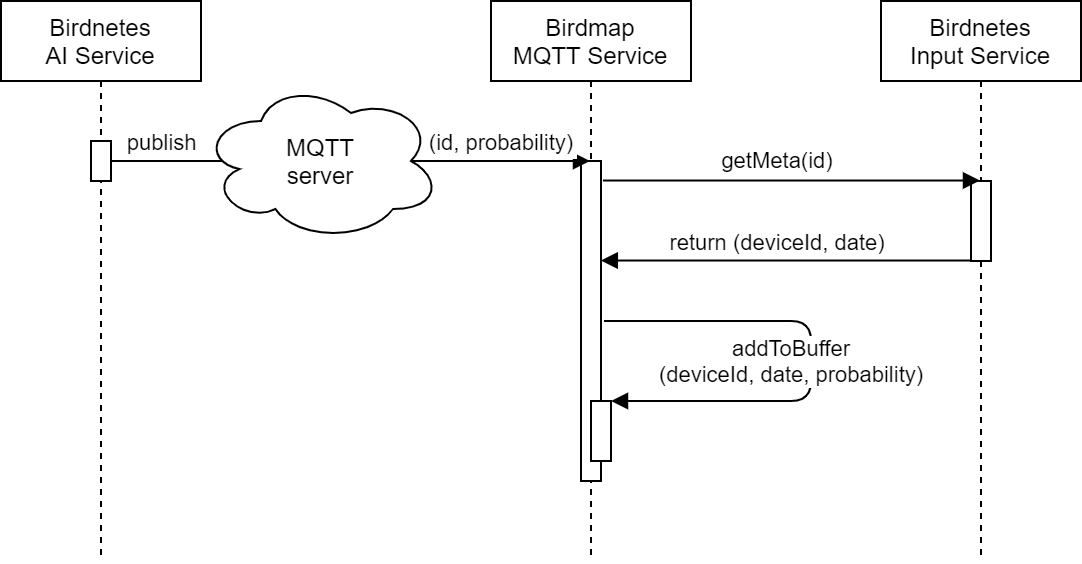
\includegraphics[width=150mm, keepaspectratio]{figures/mqtt-communication-sequence.png}
    \caption{A Birdmap MQTT szolgáltatásának szekvenciája}
    \label{fig:birdmap-mqtt-service}
\end{figure}

A puffer tartalmát másodperces gyakorisággal elküldöm a klienseknek a SignalR segítségével. 
Azért van szükség a puffer használatára, mert az MQTT-n érkezett üzenetek gyakorisága akár miliszekundum nagyságrendű is lehet. 
Míg a szerver képes is az üzeneteket feldolgozni, ha ezeket rögtön tovább küldeném a kliensek felé, azok nem biztos, hogy képesek lennének rá.

%----------------------------------------------------------------------------
\subsection{Kontrollerek}
%----------------------------------------------------------------------------
A kontrollerek határozzák meg, hogy a szerveroldalon milyen végpontokat, milyen paraméterekkel lehet meghívni, ahhoz milyen jogosultságok kellenek.
A jogosultságok kezelését a JSON Web Token-ekkel oldottam meg. A fejlasználó bejelentkezéskor kap egy ilyen token-t, 
amelyben tárolom a hozzá tartozó szerepet. A \ref{lst:devices-controller}-as listában látszik, hogy hogyan használom ezeket a szerepeket.
A kontroller végpontjait alapértelmezetten \verb+User+ és \verb+Admin+ jogosultságú felhasználó hívhatja, az online végpontot azonban csak \verb+Admin+ jogosultságú.
Hasonló képpen oldottam meg ezt a többi kontrollernél is. A \verb+User+ felhasználók csak olyan végpontokat hívhat, mely kizárolag az állapotok olvasásával jár.
Az \verb+Admin+ felhasználók hívhatnak bármilyen végpontot.

\lstset{style=sharpc, morekeywords={record, async}}
\begin{lstlisting}[caption=Az eszköz kontroller és annak "online" végpontja, label=lst:devices-controller]
    [Authorize(Roles = "User, Admin")]
    [ApiController]
    [Route("api/[controller]")]
    public class DevicesController : ControllerBase
    {
        [Authorize(Roles = "Admin")]
        [HttpPost, Route("online")]
        public async Task<IActionResult> Onlineall()
        {
            ...
        }

        ...
    }
\end{lstlisting}

Controllersw
Dtos
mapper